\section{Results and Discussion}
\label{sec:results}

\begin{table}[t]
    \centering
    \caption{Dummy main results. Higher Top-1 is better; lower NLL and ECE are
    better. Values are placeholders.}\label{tab:main-results}
    \begin{tabular}{lccc}
        \toprule
        Method & Top-1 (\%) $\uparrow$ & NLL $\downarrow$ & ECE $\downarrow$ \\
        \midrule
        Cross-entropy & 82.10 & 0.612 & 0.071 \\
        Classical KD  & 84.35 & 0.541 & 0.059 \\
        Full method   & \textbf{86.20} & \textbf{0.487} & \textbf{0.046} \\
        \bottomrule
    \end{tabular}
\end{table}


As shown in \cref{tab:main-results}, the dummy full method improves Top-1
accuracy over both the cross-entropy baseline and classical distillation. The
same trend is visualized in \cref{fig:results}. These values are deliberately
synthetic and must not be interpreted as experimental evidence.

\begin{figure}[t]
    \centering
    \definecolor{barblue}{HTML}{4C78A8}
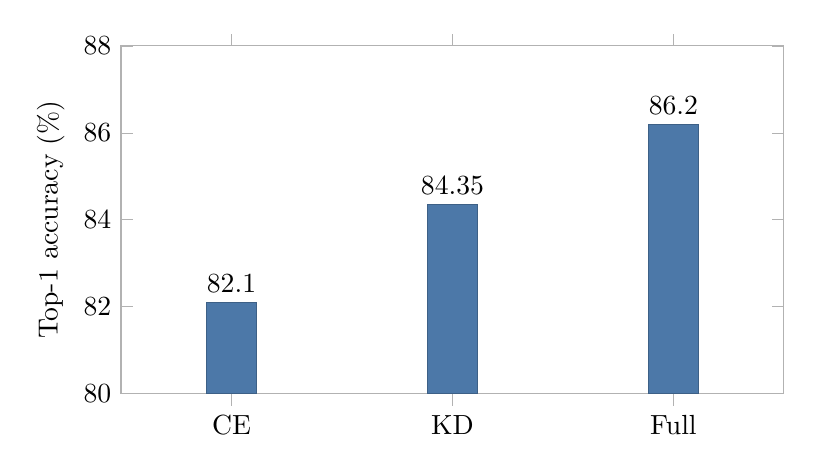
\begin{tikzpicture}
\begin{axis}[
    ybar,
    width=10cm,
    height=6cm,
    ymin=80,
    ymax=88,
    ylabel={Top-1 accuracy (\%)},
    symbolic x coords={CE,KD,Full},
    xtick=data,
    nodes near coords,
    nodes near coords align={vertical},
    bar width=18pt,
    axis line style={gray!60},
    tick style={gray!60},
    enlarge x limits=0.25
]
\addplot[fill=barblue,draw=barblue!80!black] coordinates
{(CE,82.10) (KD,84.35) (Full,86.20)};
\end{axis}
\end{tikzpicture}

    \caption{Dummy Top-1 accuracy comparison. All values are placeholders.}
    \label{fig:results}
\end{figure}

\begin{table}[t]
    \centering
    \caption{Dummy loss ablation. Checkmarks indicate enabled objectives.}
    \label{tab:ablation}
    \begin{tabular}{ccc c}
        \toprule
        $\mathcal{L}_{\mathrm{CE}}$ & $\mathcal{L}_{\mathrm{KD}}$ &
        $\mathcal{L}_{\mathrm{geo}}$ & Top-1 (\%) \\
        \midrule
        $\checkmark$ &              &              & 82.10 \\
        $\checkmark$ & $\checkmark$ &              & 84.35 \\
        $\checkmark$ & $\checkmark$ & $\checkmark$ & \textbf{86.20} \\
        \bottomrule
    \end{tabular}
\end{table}


The illustrative ablation in \cref{tab:ablation} separates the contribution of
output-level and geometry-level supervision. A real paper should report means,
standard deviations or confidence intervals, the number of seeds, and a
predefined checkpoint-selection protocol.
